\documentclass{article}
\usepackage[utf8]{inputenc}
\usepackage{hyperref}
\usepackage[english]{babel}
\usepackage{multicol}
\usepackage{xcolor}
\usepackage{graphicx}
\usepackage{comment}
\usepackage{titlesec}
\usepackage[parfill]{parskip}
\usepackage[T1]{fontenc}
\usepackage[left=4.5cm,right=4.5cm,top=4.5cm,bottom=4.5cm]{geometry}

\setlength{\columnsep}{1cm}


\title{Comparison of Sorting Algorithms}
\author{Armand Alexandru Balint\\}
\date{April 2021}

\begin{document}

\maketitle
\begin{abstract}
This paper presents a comparison of Bubble, Insertion, Merge, Quick, Heap and Counting sort with the sole purpose of finding the fastest algorithm to sort different types of lists. In the case of this paper, the files used were following different patterns of integers / floats such that there is every kind of list from a completely sorted array to a purely random one; the algorithms were then ran through the lists and had their results analyzed then written into graphs and afterwards compared. Theoretical aspects were presented and the algorithms were explained, then with that information, expectations were formed. The results are grouped into individual ones for each different array type. The overall results provided the solution to finding the fastest algorithm(s), neglecting the very minimal differences between the run-time of each \newline \newline \textbf{Keywords:} \footnotesize Bubble sort, Insertion sort, Heap sort, Merge sort, Counting sort, Algorithm implementations, Algorithm comparison


\end{abstract}
\normalsize
\pagebreak
\tableofcontents
\pagebreak

\section{Introduction}
A sorting algorithm is an algorithm that is given a list of elements alongside other minor details and arranges the elements of the list in an increasing or decreasing manner. Until today, a lot of such algorithms have been created, however some may be better than others. A sorting algorithm can be comparison based, such algorithms being: Bubble sort, Merge sort, Insertion sort, etc; and they can also be non comparison based, for example Radix Sort, Counting sort and Bucket Sort. The main objective of this paper is to find the fastest algorithm to sort a list and during that, we will encounter other circumstances under which some particular algorithm may work better than the others. The language used is the C language together with the GNU compiler.

\subsection{Comparison Based Sorting}
Upon the thought of sorting an array, comparison based sorting is probably the most common option due to the fact that it is mostly based on taking 2 numbers, comparing some aspect of them, most often which is bigger than the other, and based on that a conclusion will be drawn, whether it is to swap, not swap or to insert the element in another array.

\subsection{Non-Comparison Based Sorting}
Non comparison based sorting still makes use of comparisons however not as the primary operation. Each Non-Comparison based sorting algorithm has a different approach to sorting an array, therefore no common rule applies to them. For example$^{[1]}$ , Counting sort will use an auxiliary array of integers, aux of size k, aux[0] will hold the number of times the value min occurs in A, aux[1] will hold the number of times the value min+1 occurs and so on.

\subsection{The Divide-and-conquer approach}
The Divide and Conquer$^{[4]}$ approach, has the main goal of breaking a problem into sub-problems that are similar to the original problem recursively and then solving them once the sub-problems are small enough, combining the solutions to the sub-problems once finished to solve the original problem. Due to the fact that divide-and-conquer solves sub-problems recursively, each sub-problem must be smaller than the original one and there must be a base case for each sub-problem, therefore, each divide-and-conquer algorithm has three main parts: Divide the problem into multiple pieces, Conquer the sub-problems by solving them recursively via the base cases and finally, the combinations which, as expected, merge the sub-problems back into a big one.

\section{Classification}
In this paper, the classification of the algorithms will be done by comparing their run time and the specific requirements each one of them have. Thus, an algorithm will not be deemed as the "best" one if it is unable to sort a list of negative integers or other special cases.

\subsection{Execution Time Bounds}
Sorting algorithms are characterized by the big O notation. This notation indicates the highest possible complexity (which heavily impacts the run time) of the algorithm, it can also be referred to as an upper bound and the most common notations that will be used in this paper are:

\begin{itemize}
\item \textbf{O(n)} represents a linear graph and is the best time complexity a sorting algorithm can have, at least until a better algorithm is discovered. 


\item \textbf{O(n*log$_2$n)} is a slightly higher time complexity, however not by a lot, therefore this complexity is still considered efficient.


\item \textbf{O(n$^2$)} is the worst time complexity out of the 3 stated, given the fact that it is a quadratic one, therefore it making the graph scale increase enormously in the case of an increase of the input size.
\end{itemize}

However, there exist other complexities too, complexities such as:
\newline
\begin{minipage}{0.45\textwidth}
\begin{itemize}
  \item \textbf{O(1)} - constant time
  \item \textbf{O(log$_2$n)} - logarithmic time
\end{itemize}
\end{minipage}%
\hfill
\begin{minipage}{0.45\textwidth}
\begin{tabular}{p{\textwidth}}
\begin{itemize}
    \item \textbf{O(2$^{n}$)} - exponential time
    \item \textbf{O(n!)} - factorial time
\end{itemize}
\end{tabular}
\end{minipage}%


\pagebreak

\begin{center}
   \section{Working procedure of the algorithms} 
\end{center}

\begin{multicols}{2}
\titlespacing*{\subsection}
  {0pt}{4\baselineskip}{1.5\baselineskip}
  
\subsection{Bubble sort}

Invented by Iverson in 1962$^{[5]}$, Bubble sort is a comparison based sort. It is the simplest among all comparison based sort. In this, comparison is done among adjacent elements and if the top data is greater than the data below it then they are swapped$^{[2]}$. This will then be repeated a finite amount of times until the given data is completely sorted

\subsubsection{Time complexities}
\begin{itemize}
    \item Best case: \textbf{O(n)}
    \item Average case: \textbf{O(n$^2$)}
    \item Worst case: \textbf{O(n$^2$)}
\end{itemize}

\subsubsection{Extras}
\begin{itemize}
    \item Sorting in place: \textcolor{green}{Yes}
    \item Stable: \textcolor{green}{Yes}
\end{itemize}

\bigbreak \bigbreak \bigbreak \bigbreak \bigbreak \bigbreak \bigbreak \bigbreak \bigbreak \bigbreak \bigbreak \bigbreak



\subsection{Insertion sort}
Theorized by John Mauchly in 1946, Insertion sort is another simple to understand algorithm, however it can also be considered as one of the best algorithms in its family (O(n$^2$)) due to its performance and stability$^{[3]}$. It starts by creating a virtual split in the array which will create 2 dynamically changing arrays, a sorted and an unsorted one. A for loop is utilized to create an imaginary line which moves in an increasing manner after every iteration and every iteration, a while loop is used which, with the help of a key which represents the element the for loop iteration is on, will constantly keep the sorted part, sorted.
\subsubsection{Time complexities}
\begin{itemize}
    \item Best case: \textbf{O(n)}
    \item Average case: \textbf{O(n$^2$)}
    \item Worst case: \textbf{O(n$^2$)}
\end{itemize}

\subsubsection{Extras}
\begin{itemize}
    \item Sorting in place: \textcolor{green}{Yes}
    \item Stable: \textcolor{green}{Yes}
\end{itemize}


\bigbreak \bigbreak \bigbreak \bigbreak \bigbreak \bigbreak \bigbreak \bigbreak


\subsection{Merge sort}
Invented by John von Neumann in 1945, Merge sort is a Divide-and-conquer algorithm$^{[6]}$ which divides the input array into two halves, calls itself for the two halves and then, after n repetitions, sorts the small remaining sub-problems by merging them. The algorithm makes use of a basic function which calls itself recursively and splits the array into half until there is one element left in each sub-array and then a merge function is called which is used for merging two halves by coping the data into temporary arrays and later putting the temporary arrays together to form a bigger one, returning the final array and moving onto second smallest sub-array. This whole procedure is repeated until the array is sorted. 

\subsubsection{Time complexities}
\begin{itemize}
    \item Best case: \textbf{O(n*log$_2$n)}
    \item Average case: \textbf{O(n*log$_2$n)}
    \item Worst case: \textbf{O(n*log$_2$n)}
\end{itemize}

\subsubsection{Extras}
\begin{itemize}
    \item Sorting in place: \textcolor{red}{No}
    \item Stable: \textcolor{green}{Yes}
\end{itemize}
\bigbreak \bigbreak \bigbreak \bigbreak \bigbreak \bigbreak \bigbreak \bigbreak \bigbreak

\subsection{Quick sort}
Developed by Tony Hoare in 1959, Quick sort, similarly to Merge sort, is another Divide-and-conquer algorithm. It works by selecting a pivot element from the array and partitioning the other elements into two sub-arrays, according to whether they are less than or greater than the pivot and the sub-arrays are then sorted recursively and returned as a whole, although, if both segments are fairly large, it will be necessary to postpone the processing of one of them until the other has been fully sorted due to the recursive approach$^{[7]}$.  This strategy, however, has a weakness upon encountering bigger lists which contain only small elements due to the fact that the selection of a new pivot, different from the previous ones will be a harder to achieve task.
\subsubsection{Time complexities}
\begin{itemize}
    \item Best case: \textbf{O(n*log$_2$n)}
    \item Average case: \textbf{O(n*log$_2$n)}
    \item Worst case: \textbf{O(n$^2$)}
\end{itemize}

\subsubsection{Extras}
\begin{itemize}
    \item Sorting in place: \textcolor{green}{Yes}
    \item Stable: \textcolor{red}{No}
\end{itemize}

\bigbreak \bigbreak \bigbreak \bigbreak \bigbreak \bigbreak \bigbreak \bigbreak \bigbreak \bigbreak \bigbreak \bigbreak \bigbreak \bigbreak \bigbreak \bigbreak \bigbreak \bigbreak \bigbreak \bigbreak


\subsection{Heap sort}
Created by J.W.J. Williams in 1964, Heap sort is a comparison based sorting algorithm$^{[8]}$ where it  finds the greatest element and places it at the end then repeats the procedure by finding the second greatest and placing it at the end-1 position. This whole task is done through a binary heap where items are stored in a tree-like scheme where every level, at times except the last, is completely filled. By the end, we will have a complete binary tree where the parent node is greater(or smaller, depending on the sorting goal) than the values of its two children nodes.
\subsubsection{Time complexities}
\begin{itemize}
    \item Best case: \textbf{O(n*log$_2$n)}
    \item Average case: \textbf{O(n*log$_2$n)}
    \item Worst case: \textbf{O(n*log$_2$n)}
\end{itemize}

\subsubsection{Extras}
\begin{itemize}
    \item Sorting in place: \textcolor{green}{Yes}
    \item Stable: \textcolor{red}{No}
\end{itemize}

\bigbreak \bigbreak \bigbreak \bigbreak \bigbreak \bigbreak \bigbreak \bigbreak \bigbreak \bigbreak \bigbreak \bigbreak \bigbreak \bigbreak \bigbreak \bigbreak \bigbreak \bigbreak \bigbreak \bigbreak



\subsection{Counting sort}
Invented by Harold H. Seward in 1954, Counting sort is an algorithm based more on addition and subtraction rather than comparisons$^{[9]}$. It works by counting the number of objects having distinct key values and then counting the number of time each number appears in the given array, storing it as an index in a temporary array such that if it does not exist, we initialize it by giving the indexed array slot the value 1 and if it already exists, we increment it by one.
\subsubsection{Time complexities}
\begin{itemize}
    \item Best case: \textbf{O(n)}
    \item Average case: \textbf{O(n)}
    \item Worst case: \textbf{O(n)}
\end{itemize}

\subsubsection{Extras}
\begin{itemize}
    \item Sorting in place: \textcolor{red}{No}
    \item Stable: \textcolor{red}{No}
\end{itemize}

\bigbreak \bigbreak \bigbreak \bigbreak \bigbreak \bigbreak \bigbreak \bigbreak \bigbreak \bigbreak \bigbreak \bigbreak \bigbreak \bigbreak \bigbreak \bigbreak \bigbreak \bigbreak \bigbreak \bigbreak


\end{multicols}
\pagebreak


\section{The algorithm comparison}
Comparing the different sorting algorithms was done using a program written in C++ and compiled via the GNU compiler on an Intel i7 7700 processor running at 4 GHz, therefore the results achieved in this paper may differ from other results achieved by others using the same program, however the growth in each is going to be similar. 
\subsection{Comparison algorithm implementation}
First and foremost, the source code used can be found at the following link:  \href{https://github.com/Zedpaixd/SortingComparison}{https://github.com/Zedpaixd/SortingComparison}. That being said, the program will be given different types of lists, ordered by their types, which will be described further along, and will then run the lists through each sorting algorithm, using a 6 digit float precision timer which then will output the results of each algorithm on every given list. One thing worth noting is the fact that not every sorting algorithm used can sort every data type, such as floats, and in that case, they have been paired up with another algorithm which has the lowest run-time in sorting the remains of the list.
\subsection{Data types used}
The data types used in this evaluation vary from 10 to 900.000 elements and are as following:
\begin{itemize}
    \item Purely random lists
    \item Half sorted lists
    \item Almost sorted lists
    \item Sorted lists
    \item Reverse sorted lists
    \item Small number lists
\end{itemize}


\titleformat{\section}
  {\normalfont\Large\bfseries\centering}{\thesection}{1em}{}

\begin{center}
\section{Visualisation of final times}    

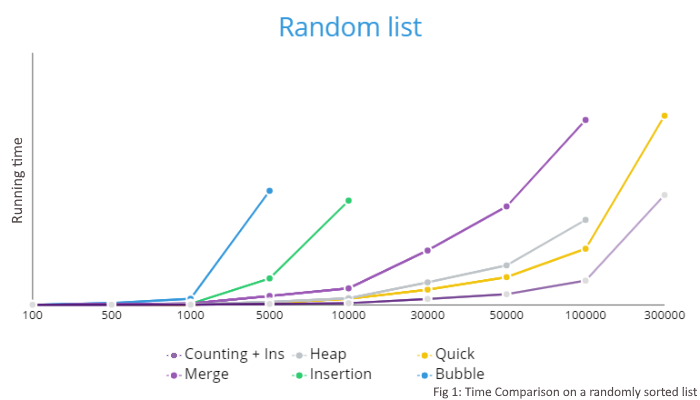
\includegraphics[width=12cm, height=6.5cm]{Random list.png}
As shown in the image above, the lowest run-time was achieved by Counting sort paired with Insertion sort. Some mandatory information is that the list was made solely out of positive integers since at the first occurrence of a negative integer, Counting sort would stop working, therefore the most optimal algorithm in this case would be Quick sort and Heap sort.
\bigbreak
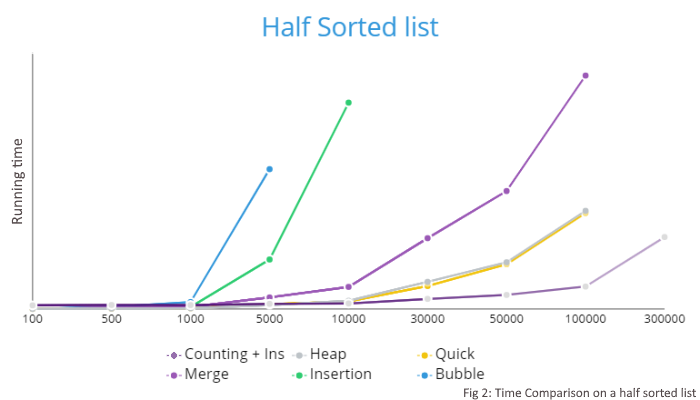
\includegraphics[width=12cm, height=6.5cm]{Half Sorted list.png}
Similar results, one thing we can notice is that Quick sort performs worse in this particular scenario, thus Heap sort will be a slightly better option in this particular scenario.
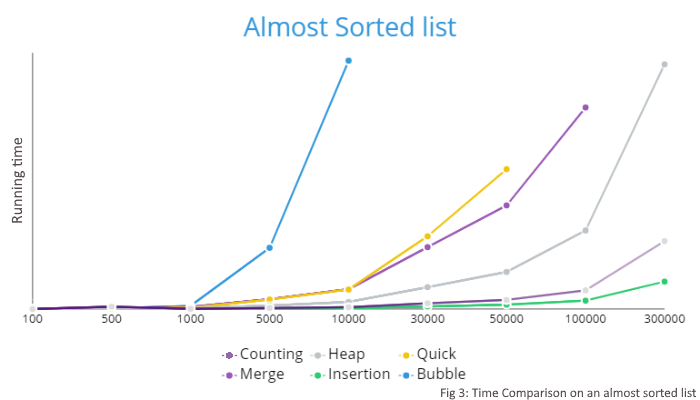
\includegraphics[width=12cm, height=6.5cm]{Almost Sorted list.png}
The first major changes can be found here, in the case of an almost sorted list, Quick sort performs increasing worse compared to other algorithms, hence why it is labeled as an unstable algorithm. However, that is not the only surprise factor, but also the fact that Insertion sort now performs better than every other algorithm tested. Keeping track of the fact that these lists do not use negative elements just so Counting sort will work properly, we can conclude that our best options in case of almost sorted lists would be Insertion sort and Heap sort.
\bigbreak
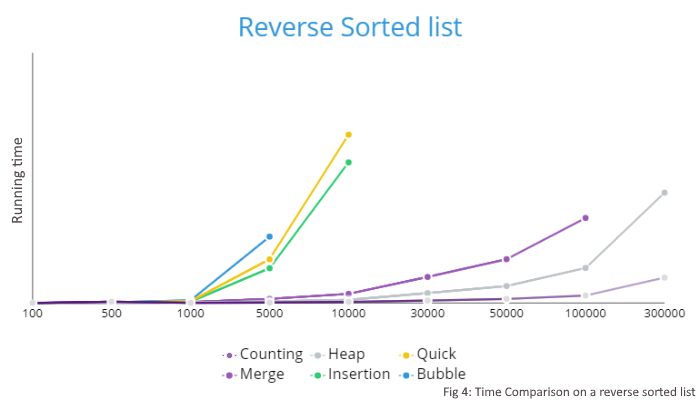
\includegraphics[width=12cm, height=6.5cm]{Reverse Sorted list_.png}
Another surprise can be noticed in the case of a reverse sorted list, which is that once again, Quick sort performs worse than many of the other algorithms tested, other than that no other unexpected outcomes can be noticed. Once again, Heap sort is one of the safest options but this time Merge sort being a fairly close second.
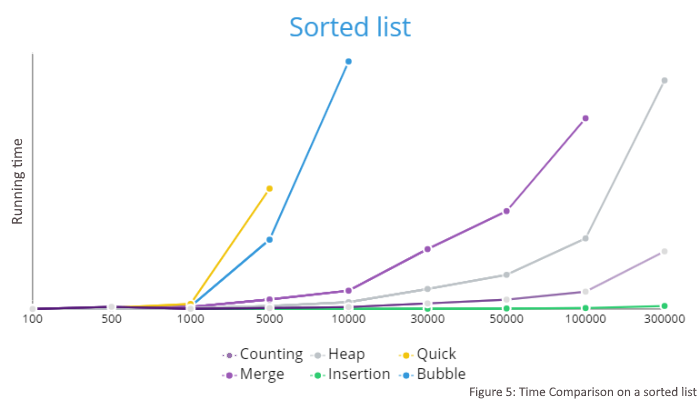
\includegraphics[width=12cm, height=6.5cm]{Sorted list.png}
Absolutely no surprises in the case of a sorted list, according to the previous time results, Quick sort being among the slowest is an expected outcome, similarly for Insertion sort being one of the fastest ones. Safest options in this case are Insertion sort and Heap sort.
\bigbreak
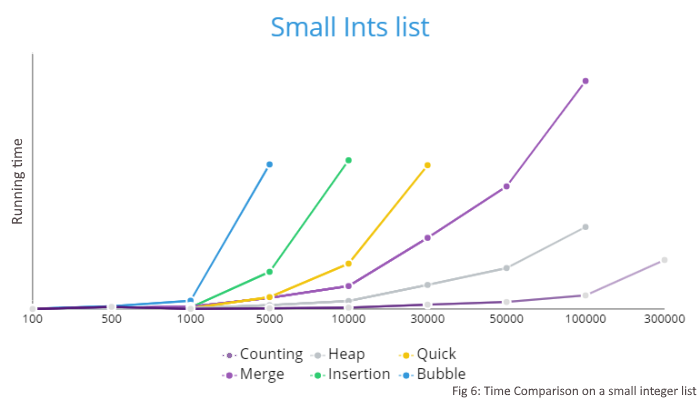
\includegraphics[width=12cm, height=6.5cm]{Small Ints list.png}
And lastly, a list created especially to ruin the run-time of Quick sort. The list is completely random, therefore the other algorithms will not have any advantage, however its unstableness in regards to small integer lists is resolute. The safest options once again shall not come as a surprise.
\end{center}

\pagebreak
\section{Conclusion}
When it comes to sorting algorithms, a "best" option is a very subjective one with lots of influential factors, starting from the kind of data given, to the content of it or even its size. That being said, the closest to a more stable option out of the tested algorithms is Heap sort, however depending on the data type, better options do exist.

\section{References}
[1] http://pages.cs.wisc.edu/~paton/readings/Old/fall08/LINEAR-SORTS.html


[2] P. K. A. S. G. Eshan Kapur, "Proposal of a two way sorting algorithm and performance with existing algorithms"Internationsl Journal of computer Science, Engineering and application, vol. 2, no. 3, 2012.


[3] Adnan Saher Mohammeda,Sahin Emrah Amrahovb, Fatih V. Celebic, "Bidirectional Conditional Insertion Sort algorithm; An efficient progress on the classical insertion sort"


[4] https://www.khanacademy.org/computing/computer-science/algorithms/merge-sort/a/divide-and-conquer-algorithms


[5] Iverson, K: A Programming Language. John Wiley, 1962.


[6] Enrico Nardelli, Guido Proietii: "Efficient unbalanced merge-sort" 29 April 2005


[7] C.A.R. Hoare: "Quicksort"


[8] Vandana Sharma, Satwinder Singh, Dr. K.S. Kahlon: "Performance Study of Improved Heap Sort Algorithm and
Other Sorting Algorithms on Different Platforms" IJCSNS International Journal of Computer Science and Network Security, VOL.8 No.4, April 2008


[9] Stijn de Gouw, Frank S. de Boer, Jurriaan Rot: "Verification of Counting Sort and Radix Sort"




\end{document}
